\section{Реализация}
\subsection{Инструменты}
Для реализации был выбран язык программирования \emph{Haskell}~\cite{haskell} и библиотека реактивного программирования \emph{reactive-banana}~\cite{reactive-banana}.
Для создания графического интерфейса приложения использовалась библиотека \emph{gtk2hs}~\cite{gtk2hs} (основанная на \emph{GTK+}~\cite{gtk}).

\subsection{Модель}
При разработке с применением ФРП в первую очередь необходимо было построить модель, описывающую
игру, выделить требуемые события и сигналы, определить зависимости между ними.

Внутренним состоянием интерфейса является информация об активных чатах, и история переписки в них.
Такую информацию удобно представить в виде отображения из JID собеседников в структуру, хранящую необходимую информацию о чате.
Данное отображение представляется в виде кусочно-постоянного сигнала, изначально равного пустому отображению.
Добавление нового собеседника происходит в двух случаях:
\begin{itemize}
    \item от собеседника приходит сообщение;
    \item пользователь двойным кликом выбирает собеседника из своего списка контактов.
\end{itemize}
Для этих двух случаев созданы отдельные события,
первое из которых наступает при поступлении соответствующей информации от библиотеки для работы с XMPP,
а наступление второго управляется при помощи \emph{gtk2hs}.
На основе этих двух событий строится итоговое событие, наступление которого обозначает, что необходимо добавить нового собеседника.
Добавленные собеседники не удаляются из отображения до конца работы программы.

Полный список событий и сигналов привден в подразделе~\ref{events_and_signals}, а их взаимосвязь отражена на рис.~\ref{network}

\subsection{События и сигналы}\label{events_and_signals}
Интерфейс приложения управляется сетью событий.
К ее входам подключены следующие события:
\begin{itemize}
    \item eInStanza --- новая строфа от сервера:
    \begin{itemize}
        \item входящее сообщение;
        \item запрос на подписку;
        \item подтверждение подписка;
        \item отказ подписки;
    \end{itemize}
    \item eOutMsg --- новое исходящее сообщение;
    \item eDoubleClick --- двойной клик пользователя на одном из элементов списка контактов.
\end{itemize}
Выводами сети логики являются следующие события:
\begin{itemize}
    \item открыть новую вкладку;
    \item отобразить новое сообщение;
    \item отправить сообщение определенному собеседнику;
    \item отправить ответ пользователя на запрос авторизации;
    \item добавить новый элемент в список контактов;
    \item удалить элемент из списка контактов;
\end{itemize}

Предварительное проектирование и явное построение модели значительно упрощает следующий этап разработки --- написание исходного кода приложения.
Фактически, требуется перевести построенную модель в термины выбранного языка программирования.

\begin{figure}[р]
\centering
\tikzstyle{IO}=[fill=yellow!20,rounded corners, draw=black!50, dashed]
\tikzstyle{event}=[draw, fill=blue!30, text width=6em, 
    text centered, minimum height=2em]
\tikzstyle{behavior}=[event, text width=10em, fill=green!20]
\tikzstyle{function}=[fill=red!20, draw=black!50,text width=8em, text centered]
\tikzstyle{condition}=[function, text width=11em, fill=black!20]
\tikzstyle{arr}=[>=stealth',semithick]
\tikzstyle{tmp}=[inner sep=0,minimum size=0]
\tikzstyle{op}=[fill=blue!20,rounded corners,minimum height=2em, text centered]
\tikzstyle{nod}=[circle,fill=black!100, inner sep=0, minimum size=2.5, draw=black!100]

\def\defw{5em}
\def\defh{1.5em}
\def\shift{0.5cm}

\tikzstyle{def}=[minimum width=\defw, minimum height=\defh, text width=\defw]

\begin{tikzpicture}
    \node               (inputLabel)                           {Input};
    \node[event]        (eInStanza)           [below=of inputLabel]                   {eInStanza};
    \node[event]        (eOutMsg)          [below=of eInStanza, yshift=-3.25cm]   {eOutMsg};
    \node[event]        (eDoubleClick)     [below=of eOutMsg, yshift=-2.3cm]  {eDoubleClick};
    \begin{pgfonlayer}{background}
        \node[IO] (input)            [fit = (inputLabel) (eInStanza) (eOutMsg) (eDoubleClick)] {};
    \end{pgfonlayer}

    \node               (procInStanzaLabel)    [right=of inputLabel, xshift=1.5cm]     {procInStanza};
    \node[condition]    (confirmC)          [below=of procInStanzaLabel]               {Confirm};
    \node[condition]    (refuseC)           [below=of confirmC, yshift=\shift]                     {Refuse};
    \node[condition]    (requestC)          [below=of refuseC, yshift=\shift]                      {Request};
    \node[condition]    (messageC)          [below=of requestC, yshift=-0.3cm]                     {Message};
    \begin{pgfonlayer}{background}
        \node[function] (procInStanza) [fit = (procInStanzaLabel) (messageC) (requestC) (confirmC) (refuseC)] {};
    \end{pgfonlayer}
    \draw[->, arr] (eInStanza.east) -- (eInStanza -| procInStanza.west);

    \node[behavior] (bChatMap)      [below=of procInStanza, xshift=2.5cm, yshift=-0.3cm] {bChatMap};
    \node[event] (eChatMap)         [below=of bChatMap, xshift=1cm, yshift=0.5cm] {eChatMap};
    \node[op] (op1) [left=of eChatMap, xshift=0.8cm] {<\%>};
    \node[function]   (addChat) [below=of eChatMap, xshift=-1cm, yshift=0.5cm] {addChat};
    \node[event] (eAddChat)         [left=of op1, xshift=0.5cm] {eAddChat};
    \draw[->, arr] (eAddChat) -- (op1);
    \draw[<-, arr] (op1.north) -- (op1 |- bChatMap.south);
    \draw[->, arr] (op1.south) -- (op1 |- addChat.north);
    \draw[<-, arr] (eChatMap.south) -- (eChatMap |- addChat.north);
    \draw[->, arr] (eChatMap.north) -- (eChatMap |- bChatMap.south);
    
    \node           (outputLabel)   [right=of procInStanzaLabel, xshift=6cm]   {Output};
    \node[function] (addContact)    [below=of outputLabel]                  {addContact};
    \node[function] (removeContact) [below=of addContact, yshift=\shift]                   {removeContact};
    \node[function] (procRequest)   [below=of removeContact, yshift=\shift]                {procRequest};
    \node[function] (send)          [below=of procRequest, yshift=\shift]                  {send};
    \node[function] (printMsg)      [below=of send, yshift=-0.5cm]                         {printMsg};
    \node[function] (showChat)      [below=of printMsg, yshift=-2.5cm]                     {showChat};
    \begin{pgfonlayer}{background}
        \node[IO] (output) [fit = (outputLabel) (printMsg) (addContact) (removeContact) (procRequest) (send) (showChat)] {};
    \end{pgfonlayer}
    \draw[->, arr]  (confirmC) to (addContact);
    \draw[->, arr]  (refuseC) to (removeContact);
    \draw[->, arr]  (requestC) to (procRequest);
    \draw[->, arr]  (procRequest) to (send);
    
    \node[event]    (ePrintMsg)     [right=of messageC, xshift=0.5cm]     {ePrintMsg};
    \node[op]       (union)         [below=of ePrintMsg, xshift=-0.5cm, yshift=0.5cm]    {$\cup$};
    \node[nod]      (tmpNod)        [left=of union]        {};
    \node[function] (procOutMsg)    [above=of ePrintMsg, xshift=-0.5cm, yshift=-0.8cm]       {procOutMsg};
    \draw[->, arr]  (messageC) to (ePrintMsg);
    \draw[->, arr]  (tmpNod) to (union);
    \draw[->, arr]  (tmpNod.north) -- (tmpNod |- procOutMsg.south);
    \draw[<-, arr]  (union.north) -- (union |- ePrintMsg.south);
    \node[op]       (op2)           [right=of union]        {<\%>};
    \draw[->, arr]  (union) to (op2);
    \draw[->, arr]  (op2.east) -- (op2 -| printMsg.west);
    \draw[->, arr]  (procOutMsg) to (send);
    \draw[arr] (tmpNod.west) -- (tmpNod -| eOutMsg.east);
    
    \node[function] (procDoubleClick)   [below=of addChat, xshift=-2.5cm, yshift=0.7cm]   {procDoubleClick};
    \node[event]    (eShowChat)         [right=of procDoubleClick, xshift=-0.5cm]                      {eShowChat};
    \node[op]       (op3)               [right=of eShowChat]                            {<\%>};
    \draw[->, arr]  (procDoubleClick) to (eShowChat);
    \draw[->, arr]  (eShowChat) to (op3);
    
    
    \draw[<-, arr]  (eAddChat.north) -- (eAddChat |- messageC.south);
    \draw[<-, arr]  (eAddChat.south) -- (eAddChat |- procDoubleClick.north);
    
    \node[nod]  (bTmpNod)   [right=of bChatMap, xshift=0.5cm] {};
    \draw[arr]      (bChatMap) -- (bTmpNod);
    \draw[->, arr]  (bTmpNod.north) -- (bTmpNod |- op2.south);
    \draw[->, arr]  (bTmpNod) -- (op3);
    \draw[<-, arr]  (procDoubleClick.west) -- (procDoubleClick -| eDoubleClick.east);
    \draw[->, arr]  (op3.east) -- (op3 -| showChat.west);
    \draw[arr] (-1,-11.5) -- (14,-11.5);
    
    \node[function, def] (funcText)  [below=of input, yshift=0.1cm] {Функция};
    \node[condition, def] (condText) [right=of funcText] {Условие};
    \node[event, def]    (eventText) [right=of condText] {Событие};
    \node[behavior, def] (bhvText) [right=of eventText] {Сигнал};
    \node[op, def] (opText) [right=of bhvText] {Оператор};

\end{tikzpicture}
\caption{Сеть событий пользовательского интерфейса}
\label{network}
\end{figure}

\begin{figure}[p]
\centering
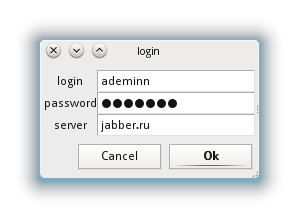
\includegraphics{pic/login.png}
\caption{Окно авторизации}
\label{pic:login}
\end{figure}

\begin{figure}[p]
\centering
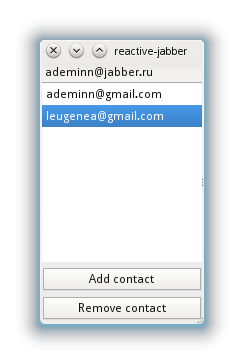
\includegraphics{pic/main.png}
\caption{Список контактов}
\label{pic:main}
\end{figure}

\begin{figure}[p]
\centering
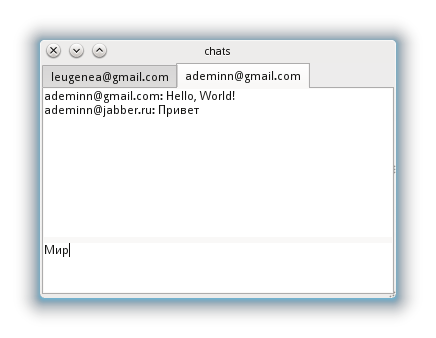
\includegraphics{pic/chats.png}
\caption{Окно чатов}
\label{pic:chats}
\end{figure}
\clearpage
\subsection{Исходный код}
\input{reactive-jabber.tex}
\input{Parser.tex}
\input{XMPPTypes.tex}
\input{XMPPMapping.tex}
\input{XMPP.tex}